\begin{figure*}[t]
\centering
\setlength{\tabcolsep}{3pt}
\begin{tabular}{@{}ccc@{}}
\textbf{BrickForma} & \textbf{BrickGPT} & \textbf{BrickNet} \\
\multicolumn{3}{@{}p{0.96\textwidth}@{}}{\small \textbf{(a) L1:} \emph{A simple chair.}} \\
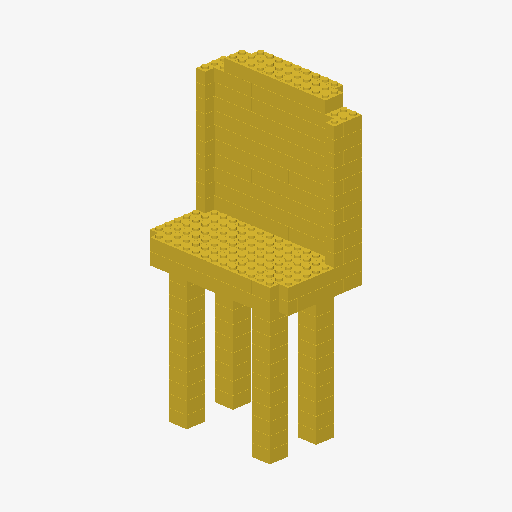
\includegraphics[width=0.136\textwidth]{figures/short_prompts/source/brickmore__chair-L1-A__stitched/01.png}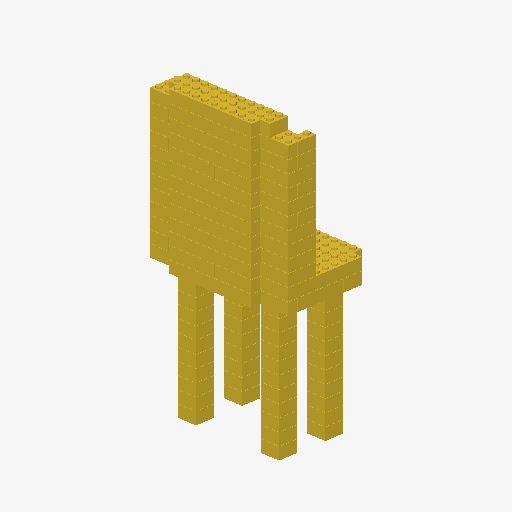
\includegraphics[width=0.136\textwidth]{figures/short_prompts/source/brickmore__chair-L1-A__stitched/05.png} & 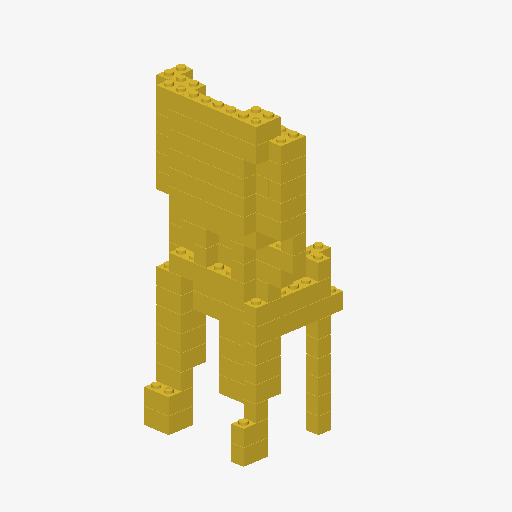
\includegraphics[width=0.136\textwidth]{figures/short_prompts/source/brickgpt__chair_L1_P01__generated/01.png}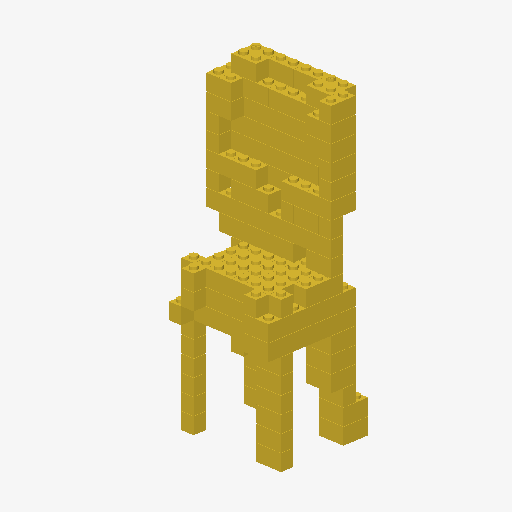
\includegraphics[width=0.136\textwidth]{figures/short_prompts/source/brickgpt__chair_L1_P01__generated/05.png} & 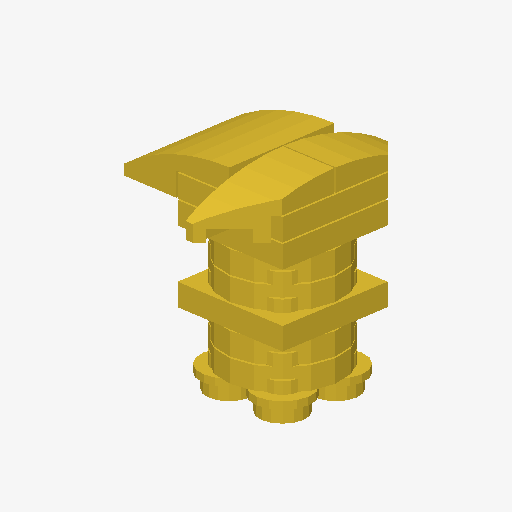
\includegraphics[width=0.136\textwidth]{figures/short_prompts/source/bricknet__chair_L1_P01__generated/01.png}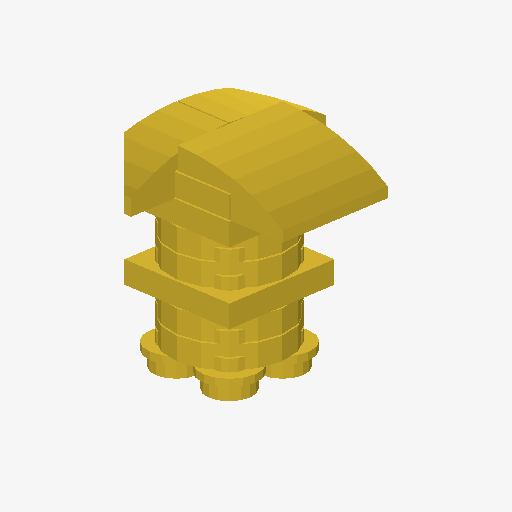
\includegraphics[width=0.136\textwidth]{figures/short_prompts/source/bricknet__chair_L1_P01__generated/05.png} \\[0pt]
\multicolumn{3}{@{}p{0.96\textwidth}@{}}{\small \textbf{(b) L1:} \emph{A compact four-door car.}} \\
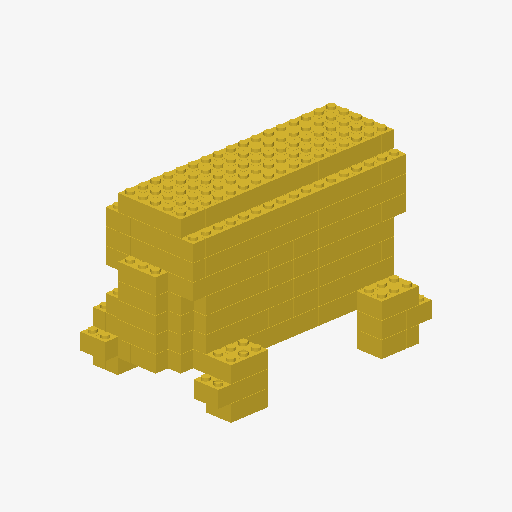
\includegraphics[width=0.136\textwidth]{figures/short_prompts/source/brickmore__car-L1V2__stitched/01.png}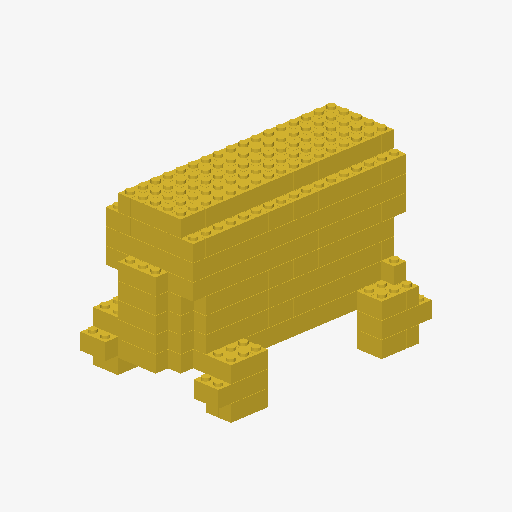
\includegraphics[width=0.136\textwidth]{figures/short_prompts/source/brickmore__car-L1V2__stitched/05.png} & 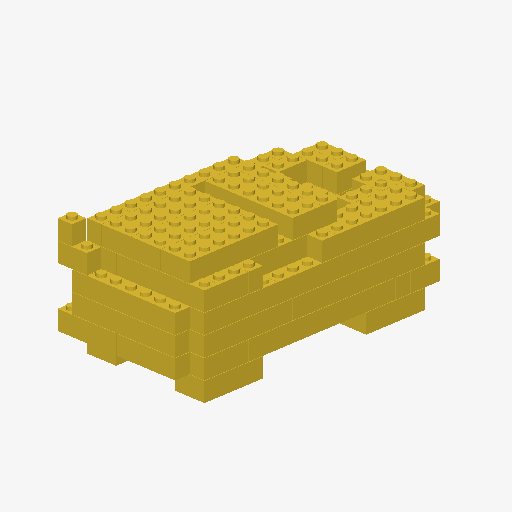
\includegraphics[width=0.136\textwidth]{figures/short_prompts/source/brickgpt__car_L1_P01__generated/01.png}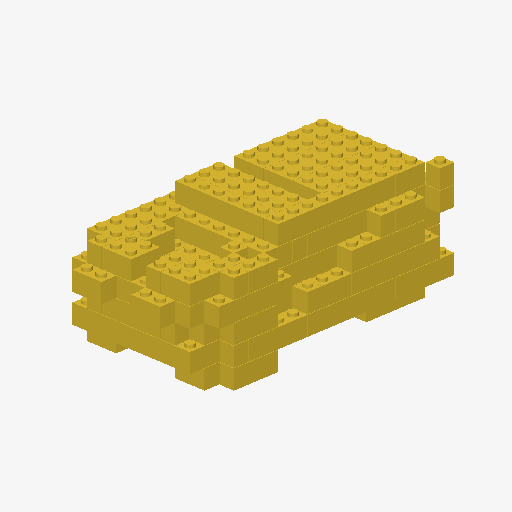
\includegraphics[width=0.136\textwidth]{figures/short_prompts/source/brickgpt__car_L1_P01__generated/05.png} & 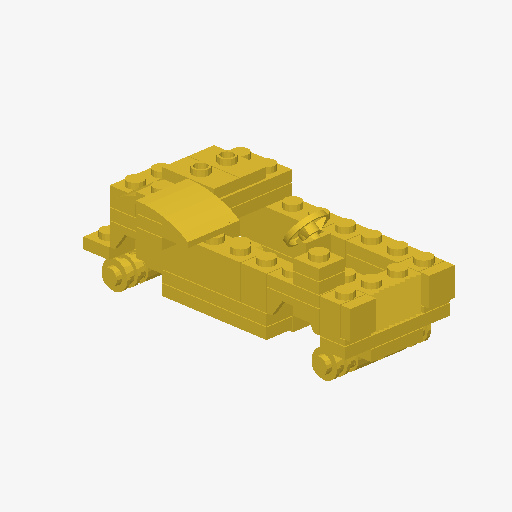
\includegraphics[width=0.136\textwidth]{figures/short_prompts/source/bricknet__car_L1_P01__generated/01.png}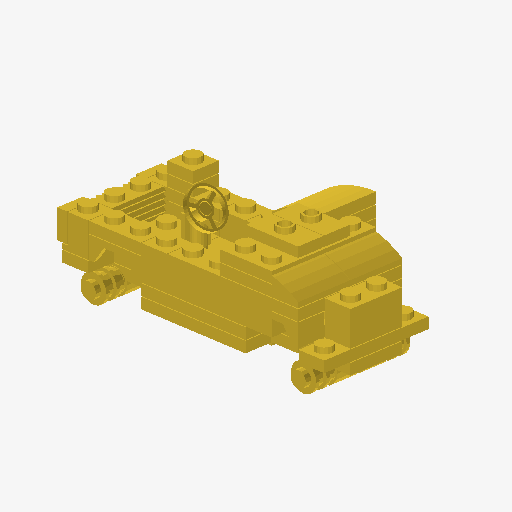
\includegraphics[width=0.136\textwidth]{figures/short_prompts/source/bricknet__car_L1_P01__generated/05.png} \\[0pt]
\multicolumn{3}{@{}p{0.96\textwidth}@{}}{\small \textbf{(c) L2:} \emph{A straight bench with a plank top and chunky leg blocks.}} \\
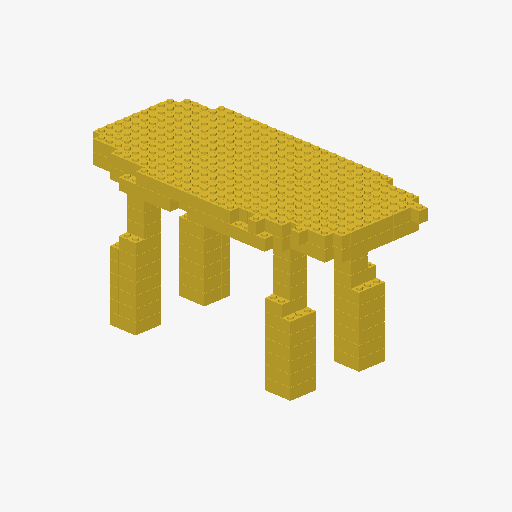
\includegraphics[width=0.136\textwidth]{figures/short_prompts/source/brickmore__bench-L2V4__stitched/01.png}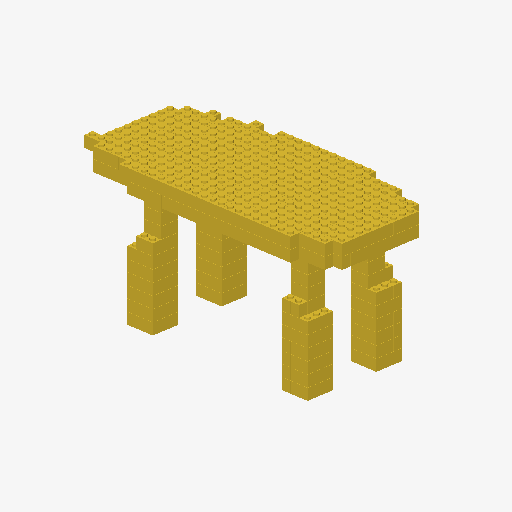
\includegraphics[width=0.136\textwidth]{figures/short_prompts/source/brickmore__bench-L2V4__stitched/05.png} & 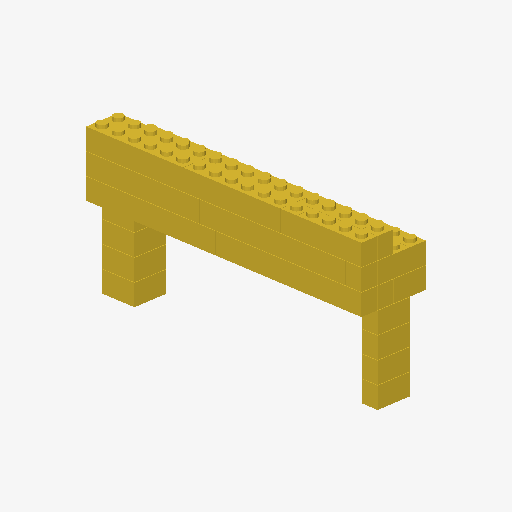
\includegraphics[width=0.136\textwidth]{figures/short_prompts/source/brickgpt__bench_L2_P01__generated/01.png}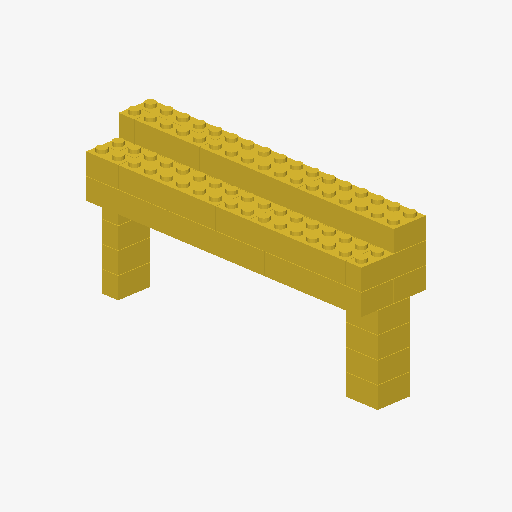
\includegraphics[width=0.136\textwidth]{figures/short_prompts/source/brickgpt__bench_L2_P01__generated/05.png} & 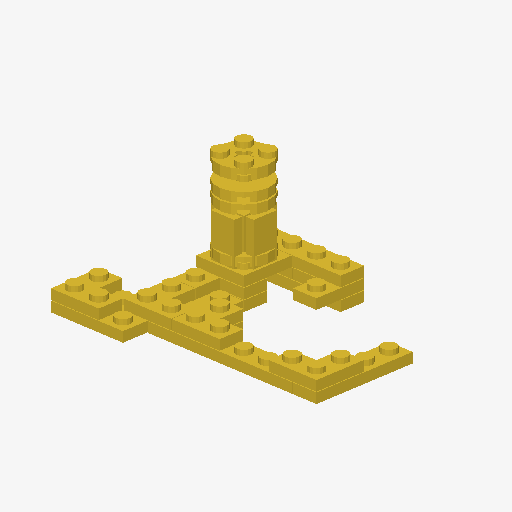
\includegraphics[width=0.136\textwidth]{figures/short_prompts/source/bricknet__bench_L2_P01__generated/01.png}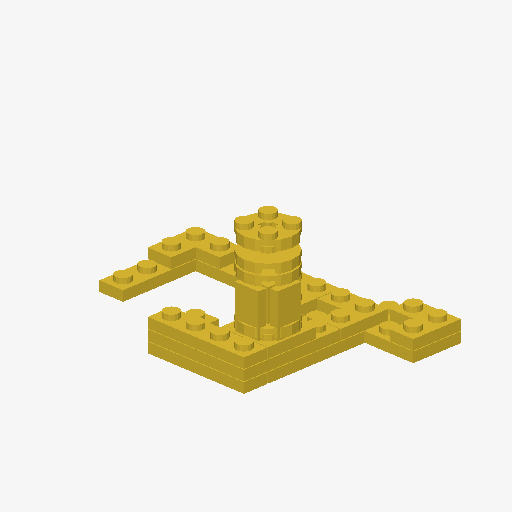
\includegraphics[width=0.136\textwidth]{figures/short_prompts/source/bricknet__bench_L2_P01__generated/05.png} \\[0pt]
\multicolumn{3}{@{}p{0.96\textwidth}@{}}{\small \textbf{(d) L2:} \emph{A rounded camera carries a circular lens at the front. The barrel connects to its body, the grip is on the right side, and the shutter and viewfinder sit on top.}} \\
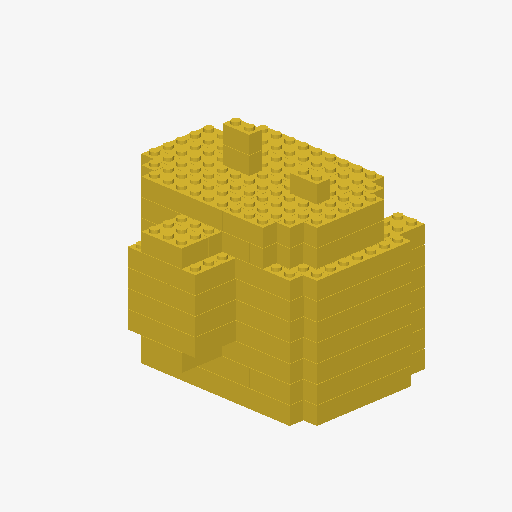
\includegraphics[width=0.136\textwidth]{figures/short_prompts/source/brickmore__camera_L2_P1_G__stitched/01.png}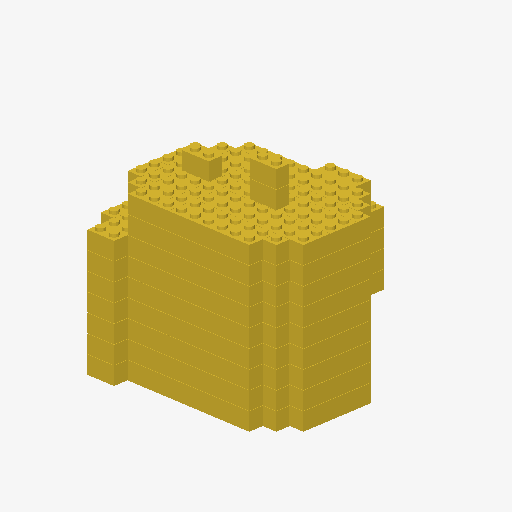
\includegraphics[width=0.136\textwidth]{figures/short_prompts/source/brickmore__camera_L2_P1_G__stitched/05.png} & 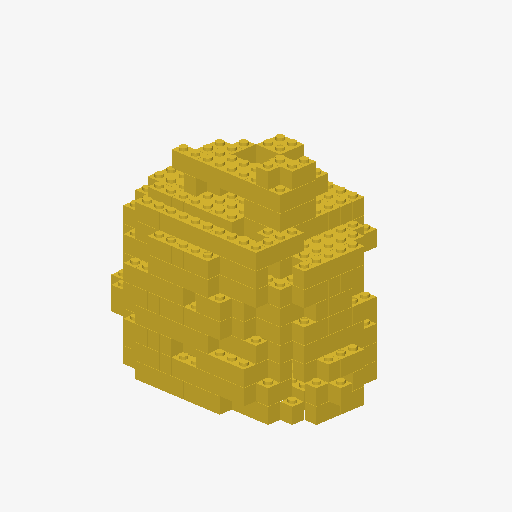
\includegraphics[width=0.136\textwidth]{figures/short_prompts/source/brickgpt__camera_L2_P01__generated/01.png}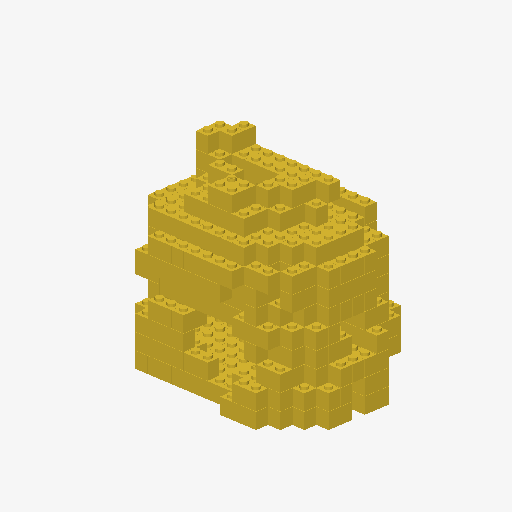
\includegraphics[width=0.136\textwidth]{figures/short_prompts/source/brickgpt__camera_L2_P01__generated/05.png} & 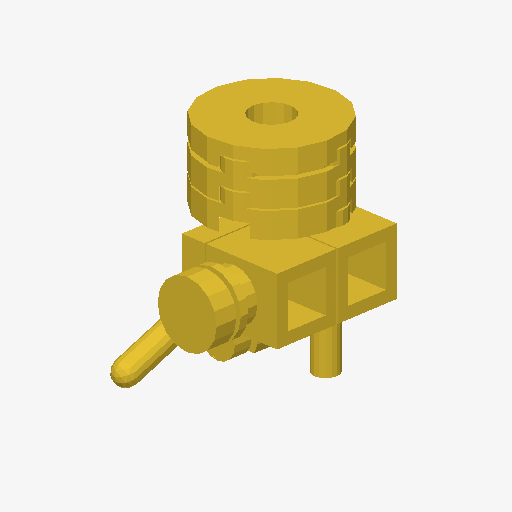
\includegraphics[width=0.136\textwidth]{figures/short_prompts/source/bricknet__camera_L2_P01__generated/01.png}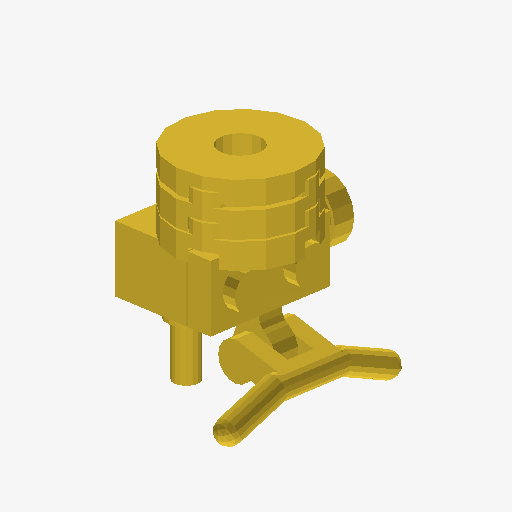
\includegraphics[width=0.136\textwidth]{figures/short_prompts/source/bricknet__camera_L2_P01__generated/05.png} \\[0pt]
\end{tabular}
\caption{Matched short-prompt examples from the main comparison. Each row uses the same prompt across all three systems and displays the same two archived camera azimuths ($45^\circ$, $225^\circ$), with $25^\circ$ elevation and uniform yellow rendering. BrickForma uses the fixed retiled main-comparison output in these four cases. Chair and bench illustrate higher BrickForma VQAScore; car and camera retain counterexamples where BrickNet has a higher VQAScore. Examples illustrate variation across cases and do not estimate a success rate.}
\label{fig:short-prompts}
\end{figure*}
